\documentclass[]{article}

\usepackage{amsmath}
\usepackage{graphicx}
\graphicspath{ {./results/} }

\title{Model CW}

\begin{document}

\maketitle

\section{Introduction}

\section{Regression}

The role of regression is to generate a model, which represents the realtionship
between the given data's independant variable and depent variable. Throughout
the code we used matrix form to calculate the model. This works by reducing the
error (residual) between the given values of $y$ and the values of y predicted by the model
$\hat{y}$. The predicted values of y are caluated by mutiplying X. X is formed
by representing the terms from the model, which for polynomial models is the
Vandermonde matrix (shown below for size n).

\begin{equation}
  X = 
  \begin{bmatrix}
    1   & x_1   & ... & {x_1}^n     \\
    1   & {x_2} & ... & {x_2}^n  \\
    ... & ...   & ... & ...     \\
    1   & {x_n} & ... & {x_n}^n  
  \end{bmatrix}
\end{equation}

For a perfect model, $y = \hat{y} = Xa$. However in most cases the given data
will not match perfectly to a model and therefore the aim is to reduce
the square error between the given $y$ values and those predicted by our model.
The value for this error (residual) can be represetned by

\begin{equation}
  r = {\mid \mid y - Xa \mid \mid}^2
\end{equation}

Minimising this vector, gives the least squares for the model and can be
represetned by this foruma.

\begin{equation}
  a = (X^T X)^{-1}X^Ty
\end{equation}

This equation will give the minimsed error for the least squares and therefore
the best model of the given type.

\section{Finding the best model}

When searching for the best model, we are looking for a model which is
generalised to the trend of the given data rather than the model with the lowest error. For a model to be
generalised it must represnt the trend of the data meaning adding more data
points from the same source would fit into the model. When a model is not
general but has a low error it is known as over-fitting. To avoid overfitting, the given data was seperated
into two groups, the training data and the testing data. The training data was
used to generate the least squares for each type of model. The least squares
generated by the training data were then used to calucalte the y values for the
testing set and the square error calucalte by the following equation

\begin{equation}
  \Sigma (y - \hat{y})^2
\end {equation}

where $y$ are the actual y values from the testing set and the $\hat{y}$ are
those calulated from the least squares generated by the training set. This
process was repeated 50 times, summing the errors for each model
type each time. The model with the lowest total error would then give the most
generalised model for the given data as the error between
the newly added data from the same source (the testing data) was low.

\section{Results}

\begin{figure}[th!]
  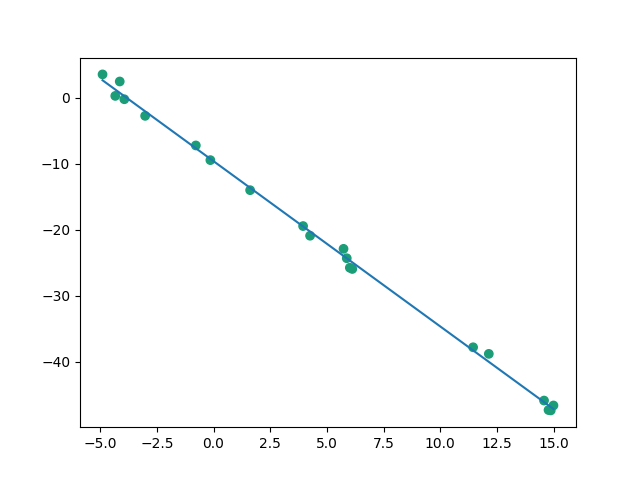
\includegraphics[scale=0.5]{noise.png}
  \centering
  \caption {Results from data set noise1}
  \label{fig:noise1}
\end{figure}

The results from \ref{fig:noise1}, show that a generalised model is gernerated. If
the model with the lowest error was used instead, we would expect the model with
a higher number of features. Instead we get a higher error but a model which
more generaly represents the given data.

\begin{figure}[!tbph]
  \centering
  \begin{minipage}[b]{0.45\textwidth}
    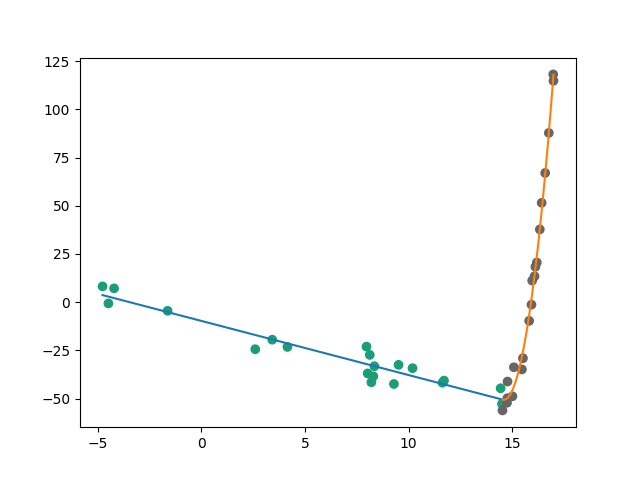
\includegraphics[width=\textwidth]{noise2.png}
    \caption {Results from data set noise2}
    \label{fig:noise2}
  \end{minipage}
  \hfill
  \begin{minipage}[b]{0.45\textwidth}
    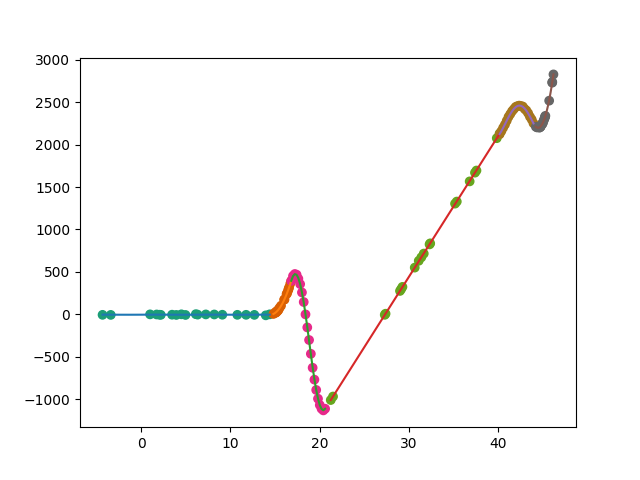
\includegraphics[width=\textwidth]{adv3.png}
    \caption {Results from data set adv3}
    \label{fig:adv3}
  \end{minipage}

\end{figure}


The results from \ref{fig:adv3} show the use of types of models. The
3rd set of 20 points is moddeled by  





\end{document}

I this coursework I implemented 3 possible funciton types: exponential,
polynomial and sinusoidal.